% +------------------------------------------------------------------------+
% | Reference manual page: Triangulation_2.tex
% +------------------------------------------------------------------------+
% | 17.03.2010   Nico Kruitof
% | Package: Periodic_2_triangulation_2
% | 
\RCSdef{\RCSTriangulationRev}{$Id$}
\RCSdefDate{\RCSTriangulationDate}{$Date$}
% |
%%RefPage: end of header, begin of main body
% +------------------------------------------------------------------------+


\ccModifierCrossRefOff
\begin{ccRefClass}{Periodic_2_triangulation_2<Traits,Tds>}

\ccDefinition

The class \ccc{Periodic_2_triangulation_2} represents a 2-dimensional
triangulation of a point set in $\mathbb T_c^2$.

\ccInclude{CGAL/Periodic_2_triangulation_2.h}

\ccParameters
The class \ccRefName\ has  two template parameters. The first one
\ccc{Traits} is the geometric traits, it is to be instantiated by
 a model of the concept \ccc{Periodic_2TriangulationTraits_2}.

The second parameter is the triangulation data structure,
it has to be instantiated by a model of the concept
\ccc{TriangulationDataStructure_2} with some additional
functionality in faces.
By default, the triangulation data structure  is instantiated by
\ccc{CGAL::Triangulation_data_structure_2 <
                       CGAL::Triangulation_ds_vertex_base_2<Gt>,
		       CGAL::Periodic_2_triangulation_ds_face_base_2<Gt> > >}.

\ccInheritsFrom{\ccc{Triangulation_cw_ccw_2}}
This class provides the functions \ccc{cw(i)} and \ccc{ccw(i)}.

\ccTypes

\ccThree{xxxxxxxxxxxxxxxxxxxxxxxxxxxxxx}{xxxxxxxxxxxxxxxxxxxxxxxxxxxx}{} \ccThreeToTwo
\ccTypedef{typedef Traits Geom_traits;}{the traits class.}
\ccGlue
\ccTypedef{typedef Tds Triangulation_data_structure;}{the triangulation data structure type.}

\ccThree{xxxxxxxxxxxxxxxxxxxxxxxxxxxxxxxxxxxxxxxxxx}{xxxxxxxxxxxxxxxx}{} \ccThreeToTwo
\ccTypedef{typedef Geom_traits::Periodic_2_offset_2 Offset;}{}
\ccGlue
\ccTypedef{typedef Geom_traits::Iso_rectangle_2 Iso_rectangle;}{the iso rectangle type}
\ccGlue
\ccTypedef{typedef array<int, 2> Covering_sheets;}{Integer tuple to
  store the number of sheets in each direction of space.}

\ccTypedef{typedef Geom_traits::Point_2 Point;}{the point type}
\ccGlue
\ccTypedef{typedef Geom_traits::Segment_2 Segment;}{the segment type}
\ccGlue
\ccTypedef{typedef Geom_traits::Triangle_2 Triangle;}{the triangle type}


\ccTypedef{typedef std::pair< Point, Offset >
  Periodic_point;}{Represents a point-offset pair. The point in the
  pair lies in the original domain.}
\ccGlue
\ccTypedef{typedef array< Periodic_point, 2>
  Periodic_segment;}{}
\ccGlue
\ccTypedef{typedef array< Periodic_point, 3>
  Periodic_triangle;}{}

\ccTypedef{typedef Tds::Vertex Vertex;}{the vertex type.}
\ccGlue
\ccTypedef{typedef Tds::Face Face;}{the face type.}
\ccGlue
\ccTypedef{typedef Tds::Edge  Edge;} {the edge type.}

\ccTypedef{typedef Tds::size_type size_type;}
{Size type (an unsigned integral type)}
\ccGlue
\ccTypedef{typedef Tds::difference_type difference_type;}
{Difference type (a signed integral type)}

\ccThree{xxxxxxxxxxxxxxxxxxxxxxxxxxxxxxxxxxxxxxxxxx}{xxxxxxxxxxxxxxxxxx}{} \ccThreeToTwo
The vertices and faces of the triangulations are accessed through 
\ccc{handles}, 
\ccc{iterators} and \ccc{circulators}. 
The  handles are models of the concept \ccc{Handle} which basically
offers the two dereference operators \ccc{*} and \ccc{->}.
The iterators and circulators
are all bidirectional and non-mutable.
The circulators and iterators are convertible  to handles with the
same value type, so that whenever a handle appear in the parameter 
list of a function, an appropriate iterator or circulator can be passed
as well.

The edges of the triangulation can also be visited through iterators
and circulators, the edge circulators and iterators are also
bidirectional and non-mutable.

\ccTypedef{typedef Tds::Vertex_handle Vertex_handle;}
{handle to a vertex}
\ccGlue
\ccTypedef{typedef Tds::Face_handle Face_handle;}
{handle to a face}


\ccTypedef{typedef Tds::Face_iterator Face_iterator;}
{iterator over all faces.}
\ccGlue
\ccTypedef{typedef Tds::Edge_iterator Edge_iterator;}
{iterator over all edges}
\ccGlue
\ccTypedef{typedef Tds::Vertex_iterator Vertex_iterator;}
{iterator over all vertices}
\ccGlue
\ccNestedType{Unique_vertex_iterator}{iterator over the vertices whose
  corresponding points lie in the original domain, i.e.\ for each set
  of periodic copies the \ccc{Unique_vertex_iterator} iterates over
  exactly one representative.}

\begin{ccAdvanced}
  These types are defined for compatibility with the
  \ccc{Triangulation_2} class.

  \ccTypedef{typedef Face_iterator Finite_faces_iterator;} {} \ccGlue
  \ccTypedef{typedef Edge_iterator Finite_edges_iterator;} {} \ccGlue
  \ccTypedef{typedef Vertex_iterator Finite_vertices_iterator;} {} \ccGlue
  \ccTypedef{typedef Face_iterator All_faces_iterator;}{}
\end{ccAdvanced}

\ccNestedType{Face_circulator} 
{circulator over all faces incident to a given vertex.}
\ccGlue
\ccNestedType{Edge_circulator}
{circulator over all  edges incident to a given vertex.}
\ccGlue
\ccNestedType{Vertex_circulator}
{circulator over all vertices adjacent to a given vertex.}

\ccHeading{Geometric iterators:}
\ccNestedType{Periodic_triangle_iterator}{iterator over the triangles
  corresponding to faces of the triangulation.}
\ccGlue
\ccNestedType{Periodic_segment_iterator}{iterator over the segments
  corresponding to edges of the triangulation.}
\ccGlue
\ccNestedType{Periodic_point_iterator}{iterator over the points
  corresponding to vertices of the triangulation.}
\ccGlue


\ccHeading{Enums:}

The triangulation class also defines the following enum types:

To specify which case occurs when locating a point in the triangulation.\\
\ccEnum{enum Locate_type {VERTEX=0, EDGE, FACE, EMPTY};}{}
  
To specify the behavior of geometric iterators.\\
\ccEnum{enum Iterator_type {STORED=0, UNIQUE, STORED_COVER_DOMAIN,
    UNIQUE_COVER_DOMAIN};}{} 


\ccCreation
\ccCreationVariable{t}  %% choose variable name



\ccThree{xxxxxxxxxxxxxxx}{t}{} \ccThreeToTwo
\ccConstructor{Triangulation_2(const Iso_rectangle & domain =
  Iso_rectangle(0,0,1,1), const Geom_traits & traits =
  Geom_traits());}{Introduces an empty triangulation \ccVar\ with
  \ccc{domain} as original domain.  \ccPrecond{\ccc{domain} is a
    square.}}

\ccConstructor{Triangulation_2(
                   const Triangulation_2& tr);}
{Copy constructor. All the vertices and faces are duplicated.
 After the copy, \ccVar\ and \ccc{tr}
refer to different triangulations: 
 if \ccc{tr} is modified, \ccVar\ is not. }

\ccMethod{Triangulation_2 operator=(const Triangulation_2<Traits,Tds>& tr);}
{Assignment. All the vertices and faces are duplicated.
 After the assignment, \ccVar\ and \ccc{tr}
refer to different triangulations: 
 if \ccc{tr} is modified, \ccVar\ is not.}

\ccMethod{void swap(Triangulation_2& tr);}
{The triangulations \ccc{tr} and \ccVar\ are swapped.
\ccc{t.swap(tr)} should be preferred to \ccc{t} = \ccc{tr} or to
\ccc{t(tr)} if \ccc{tr} is deleted after that.}

\ccMethod{void clear();}{Deletes all faces and vertices
resulting
 in an
empty triangulation.}

%\ccFunction{void ~Periodic_2_triangulation_2();}
%{Destructor. All vertices and faces are deleted.}


\ccAccessFunctions
\ccThree{Triangulation_data_structure_2}{xxxxxxxxxxxxxxxxxxxxxxxxxx}{}\ccThreeToTwo
\ccMethod{const Geom_traits& geom_traits() const;}
{Returns a const reference to the triangulation traits object.}
\ccGlue
\ccMethod{const Triangulation_data_structure_2 & tds() const;}
{Returns a const reference to the triangulation data structure.}
\ccGlue
\ccMethod{Iso_rectangle domain() const;}
{Returns the original domain.}

\ccMethod{Covering_sheets number_of_sheets() const;}
{Returns the number of sheets of the covering space the triangulation is
  currently computed in.} 
 
The responsibility of keeping a valid triangulation belongs to the user
when using advanced operations allowing a direct manipulation of the \ccc{tds}.

\ccMethod{int dimension() const;}
{Returns the dimension of the convex hull. The dimension is zero if
  the triangulation is empty and two otherwise.}

\ccMethod{size_type number_of_vertices() const;} 
{Returns the number of vertices. Counts all vertices that are
  representatives of the same point in $\mathbb T_c^2$ as one vertex.}
\ccGlue
\ccMethod{size_type number_of_faces() const;}
{Returns the number of faces. Counts all faces that are
  representatives of the same triangle in $\mathbb T_c^2$ as one face.}
\ccGlue
\begin{ccAdvanced}
\ccThree{size_type}{xxxxxxxxxxxxxxxxxxxxxxxxxxxxxxxxxxxxxxxxxxxxx}{}\ccThreeToTwo
\ccMethod{size_type number_of_stored_vertices() const;}
{Returns the number of vertices in the data structure. This is the
  same as the number of sheets times \ccc{number_of_vertices()}. }
\ccGlue
\ccMethod{size_type number_of_stored_faces() const;}
{Returns the number of faces in the data structure. This is the
  same as the number of sheets times \ccc{number_of_faces()}. }
\end{ccAdvanced}

\ccHeading{Non const access}
\begin{ccAdvanced}
\ccThree{TriangulationDataStructure_2 &}{xxxxxxxxxxxxxxxxxxxxxxxx}{}\ccThreeToTwo
\ccMethod{Triangulation_data_structure_2 & tds();}
{Returns a reference to the triangulation data structure.}

This method is mainly a help for users implementing their own triangulation
algorithms.
\end{ccAdvanced}

\ccHeading{Non-constant-time access functions}

\ccThree{size_type}{xxxxxxxxxxxxxxxxxxxxxxxxxxxxxxxxxxxxxxxxxxxxx}{}\ccThreeToTwo
\ccMethod{size_type number_of_edges() const;}
{Returns the number of edges.  Counts all edges that are
  representatives of the same segment in $\mathbb T_c^2$ as one edge.}
\ccGlue
\begin{ccAdvanced}
\ccMethod{size_type number_of_stored_edges() const;}
{Returns the number of edges in the data structure. This is the same
  as the number of sheets times \ccc{number_of_edges()}.}
\end{ccAdvanced}


\ccHeading{Non-constant-time queries and conversions}
\ccThree{bool}{xxxxxxxxxxxxxxxxxxxxxxxxxxxxxxxxxxxxxxxxxxxxxxxxxx}{}\ccThreeToTwo
\begin{ccAdvanced}
\ccMethod{bool is_extensible_triangulation_in_1_sheet_h1() const;}
{The current triangulation remains a triangulation in the 1-sheeted
  covering space even after adding points if this method returns
  \ccc{true}. This test relies on a heuristic, i.e.\ if it answers
  \ccc{false} nothing is known. This test runs in constant-time when
  not computing in the 1-sheeted covering space. (This test uses the length
of the longest edge in the triangulation as a
criterion \cite{cgal:ct-c3pt-09}.)}

\ccMethod{bool is_extensible_triangulation_in_1_sheet_h2() const;}
{The same as \ccc{is_extensible_triangulation_in_1_sheet_h1()} but with
a more precise heuristic, i.e.\ it might answer \ccc{true} in cases in which
\ccc{is_extensible_triangulation_in_1_sheet_h1()} would not. However, it is
much less time efficient when not computing in the 1-sheeted covering
space. (This test uses the diameter of the largest empty circle in the
input point set as a criterion \cite{cgal:ct-c3pt-09}.)}
\ccGlue
\ccMethod{bool is_triangulation_in_1_sheet() const;}
{Returns \ccc{true} if the current triangulation would still be a
  triangulation in the 1-sheeted covering space, returns \ccc{false} otherwise.}

It is not recommended to interfere with the built-in covering
management. Especially a premature conversion to the 1-sheeted
covering space
might lead to problems when modifying the triangulation later.
\ccMethod{void convert_to_1_sheeted_covering();}
{Converts the current triangulation into the same periodic
  triangulation in the 1-sheeted covering space.
\ccPrecond{\ccc{is_triangulation_in_1_sheet()}}
}
\ccGlue
\ccMethod{void convert_to_9_sheeted_covering();}
{Converts the current triangulation into the same periodic
  triangulation in the 9-sheeted covering space.}
\end{ccAdvanced}


\ccHeading{Geometric access functions}
\ccThree{Periodic_segment}{xxxx}{}\ccThreeToTwo

\ccMethod{Periodic_point periodic_point(const Vertex_handle v) const;}
{Returns the periodic point given by vertex \ccc{v}. If \ccVar\ is
  represented in the 1-sheeted covering space, the offset is always
  zero. Otherwise \ccc{v} can correspond to a periodic copy outside the 
  \ccc{domain} of an input point.}
%
\ccGlue
%
\ccMethod{Periodic_point periodic_point(const Face_handle f, int i)
  const;}
%
{If \ccVar\ is represented in the 1-sheeted covering space, this
  function returns the periodic point given by the $i$-th vertex of
  face \ccc{f}, that is the point in the original domain and the
  offset of the vertex in \ccc{f}.  If \ccVar\ is represented in the
  9-sheeted covering space, this offset is possibly added to another
  offset determining the periodic copy.  \ccPrecond{$i \in
    \{0,1,2\}$}}
%
\ccGlue
%
\ccMethod{Periodic_segment periodic_segment(const Face_handle f, int
  i) const;}
% 
{Returns the periodic segment formed by the two point-offset pairs
  corresponding to the two vertices of edge \ccc{(f,i)}.
  \ccPrecond{$i \in \{0,1,2\}$}}
%
\ccGlue
%
\ccMethod{Periodic_segment periodic_segment(const Edge & e) const;}
%
{Same as the previous method for edge \ccc{e}.}
%
\ccGlue
%
\ccMethod{Periodic_triangle periodic_triangle(const Face_handle f) const;} 
%
{Returns the periodic triangle formed by the three point-offset pairs
  corresponding to the three vertices of facet \ccc{f}. }

Note that a traits class providing exact constructions should be used
in order to guarantee the following operations to be exact (as opposed
to computing the triangulation only, which requires only exact
predicates).

\ccThree{Triangle}{t.segment(Periodic_segment s) const;}{}\ccThreeToTwo
\ccMethod{Point point(const Periodic_point & pp ) const;}
{Converts the \ccc{Periodic_point} \ccc{pp} (point-offset pair) to the
  corresponding \ccc{Point} in $\mathbb R^3$.}
\ccGlue
\ccMethod{Segment segment(const Periodic_segment & s) const;}
{Converts the \ccc{Periodic_segment} \ccc{s} to a \ccc{Segment}.}
\ccGlue
\ccMethod{Triangle triangle(const Periodic_triangle & t) const;}
{Converts the \ccc{Periodic_triangle} \ccc{t} to a \ccc{Triangle}.}
\ccGlue
\ccMethod{Point circumcenter(Face_handle  f) const;}
{Compute the circumcenter of the face pointed to by f. This function
is available only if the corresponding function is provided in the
geometric traits.}


The following functions are defined for convenience:

\ccMethod{Segment segment(Face_handle f, int i) const;} {Equivalent to
  the call \ccc{t.segment(t.periodic_segment(f,i));}}
%
\ccGlue
%
\ccMethod{Segment segment(const Edge& e) const;} {Equivalent to the
  call \ccc{t.segment(t.periodic_segment(e));}}
%
\ccGlue
%
\ccMethod{Segment segment(const Edge_circulator& ec) const;}
{Equivalent to the call \ccc{t.segment(t.periodic_segment(ec->first, ec->second));}}
%
\ccGlue
%
\ccMethod{Segment
          segment(const Edge_iterator& ei) const;}
{Equivalent to the call \ccc{t.segment(t.periodic_segment(ei->first, ei->second));}}
%
\ccGlue
%
\ccMethod{Triangle triangle(Face_handle f) const;}
{Equivalent to the call \ccc{t.triangle(t.periodic_triangle(f));}}

\ccPredicates 
\ccThree{bool}{t.is_edge(Vertex_handle va, Vertex_handle vb)x}{}\ccThreeToTwo
The class \ccRefName\ provides methods to test the presence in the
triangulation of a particular feature (edge or face).

\ccMethod{bool is_edge(Vertex_handle va, Vertex_handle vb);}
{\ccc{true} if there is an edge having \ccc{va} and \ccc{vb} as
vertices.}
\ccGlue
\ccMethod{bool is_edge(Vertex_handle va, Vertex_handle vb, Face_handle& fr,
	       int & i);}
{ as above. In addition, if \ccc{true} is returned,  the edge with
vertices \ccc{va} and \ccc{vb} is the edge \ccc{e=(fr,i)} where
\ccc{fr} is a handle to the face incident to \ccc{e} and 
on the right side of  \ccc{e} oriented from \ccc{va} to \ccc{vb}.}
\ccGlue
%\ccMethod{bool includes_edge(Vertex_handle va, Vertex_handle & vb,
%		     Face_handle& fr, int & i);}
%{\ccc{true} if the line segment from \ccc{va} to \ccc{vb} includes
%an edge \ccc{e} incident to \ccc{va}. If \ccc{true}, \ccc{vb} becomes
%the other vertex of \ccc{e}, \ccc{e} is the edge \ccc{(fr,i)} where
%\ccc{fr} is a handle to the face incident to \ccc{e} and 
%on the right side \ccc{e} oriented from \ccc{va} to \ccc{vb}.}
%\ccGlue
\ccMethod{bool is_face(Vertex_handle v1, Vertex_handle v2,
  Vertex_handle v3);}
%
{\ccc{true} if there is a face having \ccc{v1}, \ccc{v2} and \ccc{v3}
  as vertices.}
%
\ccGlue
%
\ccMethod{bool is_face(Vertex_handle v1, Vertex_handle v2,
  Vertex_handle v3, Face_handle &fr);}
%
{as above. In addition, if \ccc{true} is returned, \ccc{fr} is a
  handle to the face with \ccc{v1}, \ccc{v2} and \ccc{v3} as
  vertices.}

\ccHeading{Queries}

The class \ccRefName\  provides methods to locate
a given point with respect to a triangulation. It also provides
methods to locate a point with respect to
a given face of the triangulation.

\ccThree{xxxxxxxxxxxxx}{xxxxx}{}
\ccMethod{Face_handle
          locate(const Point& query,
                 Face_handle f = Face_handle()) const;}
{If the triangulation is not empty, a face 
that contains the query in its interior or on its
 boundary is returned.\\
 If the triangulation is empty, the default constructed \ccc{Face_handle} is returned.
}

\ccMethod{Face_handle
          locate(const Point& query,
                 Locate_type& lt,
                 int& li,
                 Face_handle h =Face_handle() ) const;}
{Same as above. Additionally, the parameters \ccc{lt}
 and \ccc{li}
describe where the query point is located. 
The variable \ccc{lt} is set to the locate type of the query.
If \ccc{lt==VERTEX} 
the variable \ccc{li}
is set to the index of the vertex, and if \ccc{lt==EDGE}
\ccc{li}
is set to the index 
of the vertex opposite to the
edge. 
Be careful that \ccc{li}
has no meaning when the query type is \ccc{FACE} or when the
triangulation is $0$-dimensional.}

\ccMethod{Oriented_side
           oriented_side(Face_handle f,
                         const Point& p) const;}
{Returns on which side of the oriented boundary of \ccc{f}
the point \ccc{p} lies.}

\ccMethod{Oriented_side
 side_of_oriented_circle(Face_handle f, const Point & p);}
{Returns on which side of the circumcircle  of face \ccc{f} lies 
the point \ccc{p}. The circle is assumed to be counterclockwise
oriented, so its positive
side correspond to its bounded side.
This predicate is available only if the corresponding predicates on
points is provided in the geometric traits class.}

\ccHeading{Traversal of the Triangulation}
The periodic triangulation class provides several iterators and circulators that allow one to traverse it.

\ccHeading{Face, Edge and Vertex Iterators}

The following iterators allow the user to visit faces, edges and
vertices of the stored triangulation, i.e. in case of computing in a
multiply sheeted covering space all stored periodic copies of each
item are returned. These iterators are non-mutable, bidirectional and
their value types are respectively \ccc{Face}, \ccc{Edge} and
\ccc{Vertex}.  They are all invalidated by any change in the
triangulation.

\ccThree{Vertices_iterator}{t.vertices_begin() constx}{}
\ccMethod{Vertices_iterator vertices_begin() const;}{Starts at an arbitrary vertex}
\ccGlue
\ccMethod{Vertices_iterator vertices_end() const;}{Past-the-end iterator}

\ccMethod{Edges_iterator edges_begin() const;}{Starts at an arbitrary edge}
\ccGlue
\ccMethod{Edges_iterator edges_end() const;}{Past-the-end iterator}

\ccMethod{Faces_iterator faces_begin() const;}{Starts at an arbitrary face}
\ccGlue
\ccMethod{Faces_iterator faces_end()
const;}{Past-the-end iterator}

% use periodic_points_begin() instead
%\ccMethod{Point_iterator points_begin() const;}{}
%\ccGlue
%\ccMethod{Point_iterator points_end() const;}{Past-the-end iterator}

\ccHeading{Geometric iterators}
The following iterators allow the user to obtain geometric primitives
corresponding to faces, edges, and vertices of the triangulation.
These iterators are non-mutable, bidirectional and their value types
are respectively \ccc{Periodic_triangle}, \ccc{Periodic_segment} and
\ccc{Periodic_point}. They are all
invalidated by any change in the triangulation. If the periodic
triangulation is not computed in the 1-sheeted covering space, these iterators
can be used to retain only the geometric primitives in the original
domain. This can be controlled using the enum \ccc{Iterator_type}, see
\ccRefIdfierPage{CGAL::Periodic_2_triangulation_2::Iterator_type}. 

\begin{figure}[htbp]
\begin{ccTexOnly}
\begin{center} 
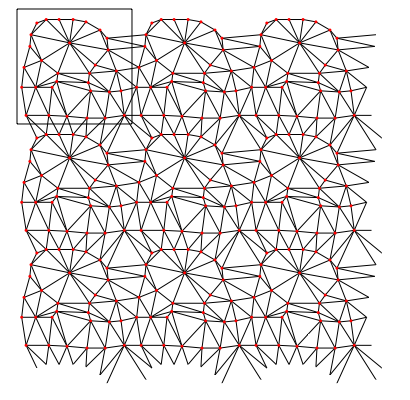
\includegraphics[width=5cm]{Periodic_2_triangulation_2_ref/it_STORED} 
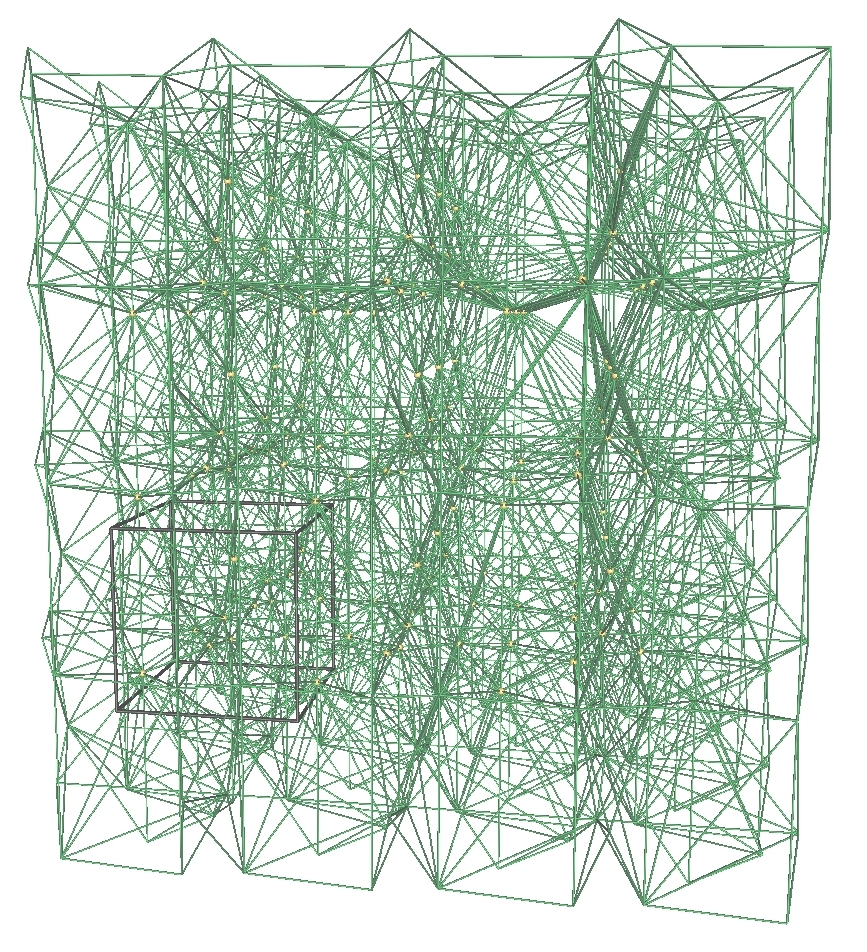
\includegraphics[width=5cm]{Periodic_2_triangulation_2_ref/it_STORED_COVER_DOMAIN}\\
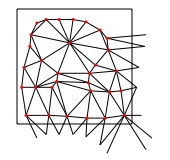
\includegraphics[width=5cm]{Periodic_2_triangulation_2_ref/it_UNIQUE} 
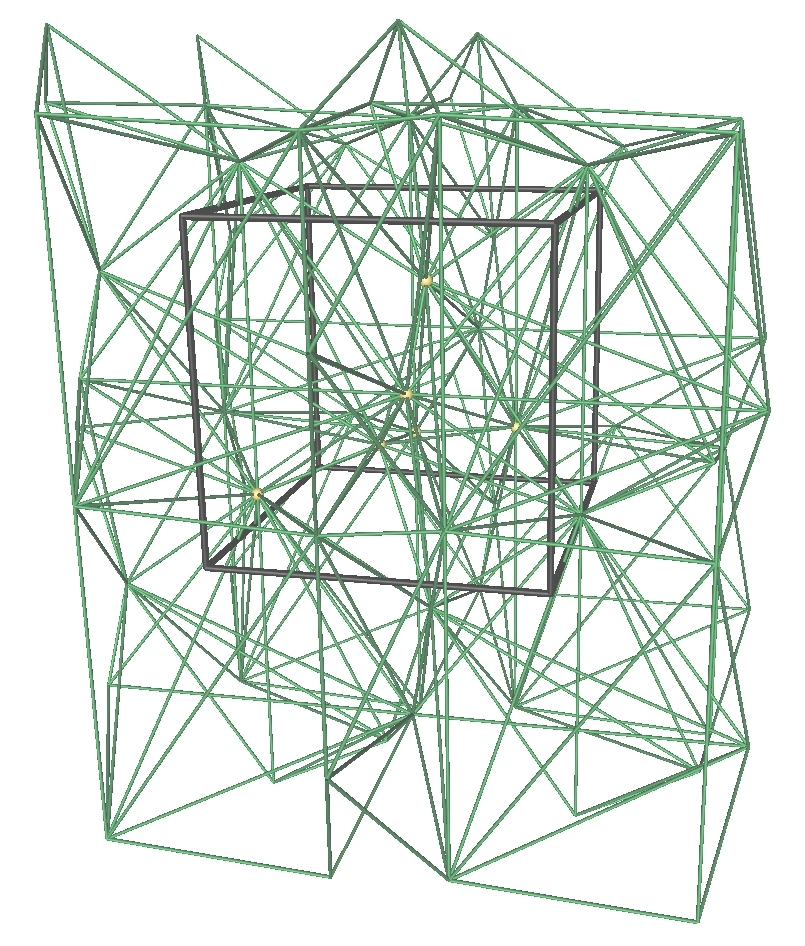
\includegraphics[width=5cm]{Periodic_2_triangulation_2_ref/it_UNIQUE_COVER_DOMAIN} 
\end{center}
\end{ccTexOnly}
\begin{ccHtmlOnly}
<CENTER>
<img border=0 src="./it_STORED_small.png" align=middle
  alt="STORED">
<img border=0 src="./it_STORED_COVER_DOMAIN_small.jpg" align=middle
  alt="STORED_COVER_DOMAIN">
<img border=0 src="./it_UNIQUE_small.png" align=middle
  alt="UNIQUE">
<img border=0 src="./it_UNIQUE_COVER_DOMAIN_small.jpg" align=middle
  alt="UNIQUE_COVER_DOMAIN">
</CENTER>
\end{ccHtmlOnly}
%
\caption{NGHK: Change images. The four different modes of the
  geometric iterators: \ccc{STORED}, \ccc{STORED\_COVER\_DOMAIN},
  \ccc{UNIQUE}, \ccc{UNIQUE\_COVER\_DOMAIN}. Note that in case of
  computing in the 1-sheeted covering space, \ccc{STORED*} and
  \ccc{UNIQUE*} give the same result.
  \label{P2Triangulation2-fig-geom_iterators}}
%
\end{figure} 

\ccThree{Periodic_triangle_iteratorx}{XXXXXXX}{}

\ccMethod{Periodic_point_iterator periodic_points_begin(Iterator_type it =
  STORED) const;}
{Iterates over the points of the triangulation. Its behavior is
  defined by the \ccc{Iterator_type} \ccc{it} as described on
  \ccRefIdfierPage{CGAL::Periodic_2_triangulation_2::Iterator_type}.}
\ccGlue
\ccMethod{Periodic_point_iterator periodic_points_end(Iterator_type it =
  STORED) const;}
{Past-the-end iterator. Note that to match another
  \ccc{Periodic_point_iterator} both must have the same
  \ccc{Iterator_type} \ccc{it}.}

\ccMethod{Periodic_segment_iterator periodic_segments_begin(Iterator_type it =
  STORED) const;}
{Iterates over the segments of the triangulation. Its behavior is
  defined by the \ccc{Iterator_type} \ccc{it} as described on
  \ccRefIdfierPage{CGAL::Periodic_2_triangulation_2::Iterator_type}.}
\ccGlue
\ccMethod{Periodic_segment_iterator periodic_segments_end(Iterator_type it =
  STORED) const;}
{Past-the-end iterator. Note that to match another
  \ccc{Periodic_segment_iterator} both must have the same
  \ccc{Iterator_type} \ccc{it}.}

\ccMethod{Periodic_triangle_iterator periodic_triangles_begin(Iterator_type it =
  STORED) const;}
{Iterates over the triangles of the triangulation. Its behavior is
  defined by the \ccc{Iterator_type} \ccc{it} as described on
  \ccRefIdfierPage{CGAL::Periodic_2_triangulation_2::Iterator_type}.}
\ccGlue
\ccMethod{Periodic_triangle_iterator periodic_triangles_end(Iterator_type it =
  STORED) const;}
{Past-the-end iterator. Note that to match another
  \ccc{Periodic_triangle_iterator} both must have the same
  \ccc{Iterator_type} \ccc{it}.}

\ccHeading{Face, Edge and Vertex Circulators}
\ccThree{Vertex_circulator}{xxx}{}
\ccThreeToTwo

The triangulation also provides circulators that allows to visit 
respectively all faces or edges incident to a given vertex
or all vertices adjacent to a given vertex.
These circulators are
non-mutable
and bidirectional.
 The \ccc{operator++} moves the circulator
counterclockwise around the vertex while
the \ccc{operator--} moves clockwise.
A face circulator is invalidated by any modification of the face pointed to.
An edge or a vertex circulator are invalidated by any modification
of one of the two faces incident to the edge pointed to.

\ccMethod{Face_circulator incident_faces(Vertex_handle v) const;}
{Starts at an arbitrary face incident
to \ccc{v}.}
\ccGlue
\ccMethod{Face_circulator incident_faces(Vertex_handle v, Face_handle f) const;}
{Starts at face \ccc{f}.
\ccPrecond Face \ccc{f} is incident to vertex \ccc{v}.}
\ccGlue
\ccMethod{Edge_circulator incident_edges(Vertex_handle v) const;}
{Starts at an arbitrary edge incident
to \ccc{v}.}
\ccGlue
\ccMethod{Edge_circulator incident_edges(Vertex_handle v, Face_handle f) const;}
{Starts at the first edge of \ccc{f} incident to 
\ccc{v}, in counterclockwise order around \ccc{v}.
\ccPrecond Face \ccc{f} is incident to vertex \ccc{v}.}
\ccGlue
\ccMethod{Vertex_circulator adjacent_vertices(Vertex_handle v) const;}
{Starts at an arbitrary  vertex adjacent to \ccc{v}.}
\ccGlue
\ccMethod{Vertex_circulator adjacent_vertices(Vertex_handle v, Face_handle f) ;}
{Starts at the first vertex of \ccc{f} adjacent  to \ccc{v}
in  counterclockwise order around \ccc{v}.
\ccPrecond Face \ccc{f} is incident to vertex \ccc{v}.}



\ccHeading{Traversal between adjacent faces}
\ccMethod{Vertex_handle  mirror_vertex(Face_handle f, int i) const;}
{returns the vertex of the $i^{th}$ neighbor of \ccc{f} that is
  opposite to \ccc{f}.
  \ccPrecond $0\leq i \leq 2$.}
\ccGlue
\ccMethod{int   mirror_index(Face_handle f, int i) const;}
{returns the index of \ccc{f} in its $i^{th}$ neighbor.
  \ccPrecond $0\leq i \leq 2$.}

\ccHeading{Modifiers}

The following operations are guaranteed to lead to a valid triangulation 
when they are applied on a valid triangulation.

\ccThree{Vertex_handle}{xxx}{}

\ccMethod{void flip(Face_handle f, int i);}{Exchanges the edge
  incident to \ccc{f} and \ccc{f->neighbor(i)} with the other diagonal
  of the quadrilateral formed by \ccc{f} and
  \ccc{f->neighbor(i)}. Flips all periodic copies of the edge when
  the triangulation is on the 9-sheeted cover.
%
  \ccPrecond {The union of the faces \ccc{f} and \ccc{f->neighbor(i)}
    form a convex quadrilateral.}}
%
\ccGlue
%
\ccMethod{Vertex_handle insert(const Point& p, Face_handle f =
  Face_handle());}
%
{Inserts point \ccc{p} in the triangulation and returns the
  corresponding vertex.\\ If point \ccc{p} coincides with an already
  existing vertex, this vertex is returned and the triangulation
  remains unchanged.\\ If point \ccc{p} is on an edge, the two
  incident faces are split in two, see
  Figure~\ref{Triangulation_ref_Fig_insert1}.\\ If point \ccc{p} is
  strictly inside a face of the triangulation, the face is split in
  three, see Figure~\ref{Triangulation_ref_Fig_insert2}.\\ If the
  triangulation is empty, the triangulation with a single vertex at
  point \ccc{p} is created.\\ The last argument \ccc{f} is an
  indication to the underlying locate algorithm of where to start.
  \ccPrecond{\ccc{p} lies in the original domain.}  }
%
\ccGlue
%
\ccMethod{Vertex_handle insert(const Point& p, Locate_type lt,
  Face_handle loc, int li );} {Same as above except that the location
  of the point \ccc{p} to be inserted is assumed to be given by
  \ccc{(lt,loc,i)} (see the description of the \ccc{locate} method
  above.)}
%
\ccGlue
%
\ccMethod{Vertex_handle push_back(const Point& p);} {Equivalent to
  \ccc{insert(p)}.}
%
\ccGlue
%
\ccMethod{template < class InputIterator > int insert(InputIterator
  first, InputIterator last);} {Inserts the points in the range
  $\left[\right.$\ccc{first}, \ccc{last}$\left.\right)$.  Returns the
  number of inserted points.  \ccPrecond The \ccc{value_type} of
  \ccc{InputIterator} is \ccc{Point} and all points lie in the
  original domain.}
%
\ccGlue
%
\ccMethod{void remove(Vertex_handle v);} {Removes the vertex from the
  triangulation. The created hole is re-triangulated, see
  Figure~\ref{Triangulation_ref_Fig_remove}.}

\begin{figure}
\begin{ccTexOnly}
\begin{center}
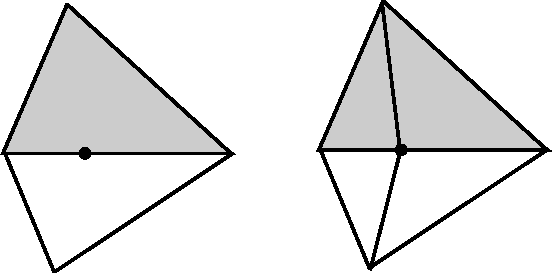
\includegraphics{Periodic_2_triangulation_2/insert1}
\end{center}
\end{ccTexOnly}


\begin{ccHtmlOnly}
<CENTER>
<img border=0 src="./insert1.gif" align=middle alt="Insertion in an edge">
</CENTER>
\end{ccHtmlOnly}

\caption{Insertion of a point on an edge.
\label{Triangulation_ref_Fig_insert1}}
\end{figure}




\begin{figure}
\begin{ccTexOnly}
\begin{center}
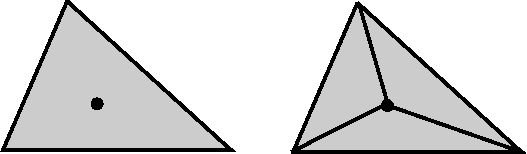
\includegraphics{Periodic_2_triangulation_2/insert2}
\end{center}
\end{ccTexOnly}

\begin{ccHtmlOnly}
<CENTER>
<img border=0 src="./insert2.gif" align=middle alt="Insertion in a Face">
</CENTER>
\end{ccHtmlOnly}

\caption{Insertion in a face.
\label{Triangulation_ref_Fig_insert2}}

\end{figure}


\begin{figure}
\begin{ccTexOnly}
\begin{center}
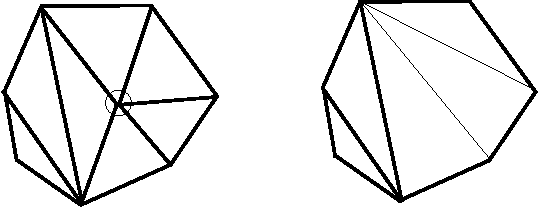
\includegraphics{Periodic_2_triangulation_2/remove}
\end{center}
\end{ccTexOnly}

\begin{ccHtmlOnly}
<CENTER>
<img border=0 src="./remove.gif" align=middle alt="Remove">
</CENTER>
\end{ccHtmlOnly}

\caption{Removal
\label{Triangulation_ref_Fig_remove}}
\end{figure}

\begin{ccAdvanced}
The following member functions offer more specialized versions of the
insertion or removal operations to be used when one knows to be in the
corresponding case.

\ccMethod{Vertex_handle insert_first(const Point& p);} 
{Inserts the first vertex.}
\ccMethod{Vertex_handle insert_in_face(const Point& p, Face_handle f);} {Inserts vertex \ccc{v} in face
\ccc{f}. Face \ccc{f} is modified,
two new faces are created. If the triangulation contains periodic copies, a point is inserted in all periodic copies.
\ccPrecond{The point in vertex \ccc{v} lies inside face \ccc{f}.}}
\ccMethod{Vertex_handle insert_in_edge(const Point& p, const Offset &o, Face_handle f, int i);} 
{Inserts vertex v in edge \ccc{i} of \ccc{f}. If the triangulation contains periodic copies, a point is inserted in all periodic copies.
\ccPrecond{The point in vertex \ccc{v} lies on the edge opposite to 
the vertex \ccc{i} of face \ccc{f}.}}

\ccMethod{void remove_degree_3(Vertex_handle v);}
{Removes a vertex of degree three. Two of the incident faces are
  destroyed, the third one is modified.  \ccPrecond{Vertex \ccc{v} is
    a vertex with degree three.}}  \ccMethod{void
  remove_first(Vertex_handle v);}{Removes the unique vertex in the
  triangulation.}

The following functions are mainly intended to be used in conjunction
with the \ccc{find_conflicts()} member functions of Delaunay and constrained 
Delaunay triangulations to perform insertions.

\ccMethod{   template<class EdgeIt>
   Vertex_handle star_hole( Point p, 
 			      EdgeIt edge_begin,
 			      EdgeIt edge_end);}
{creates a new vertex \ccc{v} and use it to star the hole 
whose boundary is described  by the sequence of edges \ccc{[edge_begin, 
edge_end]}. Returns a handle to the new vertex.}

\ccMethod{
   template<class EdgeIt, class FaceIt>
   Vertex_handle star_hole( Point p, 
 			      EdgeIt edge_begin,
 			      EdgeIt edge_end,
 			      FaceIt face_begin,
 			      FaceIt face_end);}
{same as above, except that the  algorithm 
first recycles faces in the sequence \ccc{[face_begin, 
face_end]} 
and create new ones only when the sequence is exhausted.}
\end{ccAdvanced}

\begin{ccAdvanced}
  \ccMethod{void set_domain(const Iso_rectangle dom);} {Changes the
    domain. Note that this function calls \ccc{clear()}, i.e., it
    erases the existing triangulation. }
\end{ccAdvanced}


\ccHeading{Miscellaneous}

\ccThree{size_t}{t.flippable(Face_handle f, int i);}{}
%
\ccMethod{int ccw(int i) const;} {Returns $i+1$ modulo 3.\ccPrecond
  $0\leq i \leq 2$.}
%
\ccGlue
%
\ccMethod{int cw(int i) const;} {Returns $i+2$ modulo 3.\ccPrecond
  $0\leq i \leq 2$.}
%
\ccGlue
%
\ccMethod{void flippable(Face_handle f, int i);} { Returns whether the
  union of the faces \ccc{f} and \ccc{f->neighbor(i)} form a convex
 quadrilateral.}
%
\ccGlue
%
\ccMethod{size_t degree(Vertex_handle v);} { Returns the degree of the
  vertex \ccc{v}}

\begin{ccAdvanced}

\ccHeading{Checking}
The responsibility of keeping a valid triangulation
belongs to the users if advanced operations are used.
Obviously the advanced user, who implements higher levels operations
may have to make a triangulation invalid at some times. The following
method is provided to help the debugging.

\ccMethod{bool
          is_valid(bool verbose = false, int level = 0) const;}
{Checks the combinatorial validity of the triangulation and
also the validity of its geometric embedding.
 This method is  mainly a debugging help
for the users of advanced features.
}
\end{ccAdvanced}


\ccHeading{I/O}


The I/O operators are defined for \ccc{iostream}.  The format for the
iostream is an internal format.

\ccInclude{CGAL/IO/ostream_2.h}

\ccThree{ostreamxx}{ostream}{}
%
\ccFunction{ostream& operator<<(ostream& os, const
  Periodic_2_triangulation_2<Traits,Tds>& T);} {Writes the
  triangulation \ccVar\ into the stream \ccc{os}.  \ccPrecond The
  output operator must be defined for \ccc{Point}.}
%
\ccGlue
%
\ccFunction{istream& operator>>(istream& is,
  Triangulation_2<Traits,Tds>& T);} {Reads a triangulation from stream
  \ccc{is} and assigns it to \ccVar. \ccPrecond The input operator
  must be defined for \ccc{Point}.}


The information in the \ccc{iostream} is:
\begin{itemize}
\item the original domain
\item the number of sheets of the covering space as in
  \ccc{number_of_sheets()}
\item the number of vertices
\item the non-combinatorial information of vertices (point
  resp. point-offset pairs, etc.)
\item the number of faces
\item the indices of the vertices of each face
\item the indices of the neighbors of each face, where the index
  corresponds to the preceding list of faces
\item the offsets corresponding to the vertices of the faces
\item the non-combinatorial information of each face
\end{itemize}

CGAL also provides a stream operator \ccc{<<} to draw triangulations
for \ccc{CGAL::Qt_widget}, the Qt based graphic package.
These operators require the include statement: \\
\ccInclude{CGAL/IO/Qt_widget_Triangulation_2.h}\\
See the \ccc{Qt_widget} class.

%\ccThree{Line_face_circulator}{T.line_walk(Point p, }{}
%\ccHeading{Line Face Circulator}
%
%The triangulation defines a circulator that allows
%to visit all faces that are intersected by a line. 
%  face  \ccc{f} is 
%considered has being intersected by 
% the oriented line \ccc{l} if either:
%\begin{itemize}\ccTexHtml{\itemsep0pt}{}
%\item 
%\ccc{f} is a finite face whose interior intersects \ccc{l}, or
%\item
% \ccc{f} is a finite face with  an edge collinear with \ccc{l} and lies
%to the left of \ccc{l}, or
%\item
%\ccc{f} is an infinite face incident to a  convex hull edge 
%whose interior is intersected
%by \ccc{l}, or
%\item
%\ccc{f} is an infinite face incident to a  convex hull vertex
%lying on  \ccc{l} and the finite edge of \ccc{f}
%lies to the left of \ccc{l}. 
%\end{itemize}
%The circulator has a singular value if  the line \ccc{l}
%intersect no finite face of the triangulation.
%This circulator is
%non-mutable and bidirectional. Its value type is \ccc{Face}.
%
%\ccMethod{Line_face_circulator
%          line_walk(const Point& p,
%                    const Point& q,
%                    Face_handle f = Face_handle()) const;}
%{ This function returns a circulator that allows to visit the 
% faces intersected by the line \ccc{pq}. 
%If there is no such face the circulator has a singular value.\\
% The starting point of the circulator is the face \ccc{f}, or
% the first finite face traversed by \ccc{l} , if
% \ccc{f} is omitted. \\
%  The circulator wraps around the \ccc{infinite_vertex}:
%after the last traversed finite face, it steps through the infinite face adjacent
%to this face then through the infinite face adjacent to the first
%traversed finite face then through the first finite traversed face
%again.
%\ccPrecond The triangulation is not empty.
%\ccPrecond Points \ccc{p} and \ccc{q} must be different points inside the original domain.
%\ccPrecond If \ccc{f != NULL}, it must point to a finite face
% and the point \ccc{p} must be
%inside or on the boundary of \ccc{f}.}
%
%Figure~\ref{Triangulation_ref_Fig_Line_face_circulator} illustrates which finite faces are enumerated. Lines
%$l_1$ and $l_2$ have no face to their left. Lines $l_3$ and $l_4$
%have faces to their left. Note that the finite faces that are only vertex
%incident to lines $l_3$ and  $l_4$ are not enumerated.
%
%\begin{figure}
%\begin{ccTexOnly}
%\begin{center}  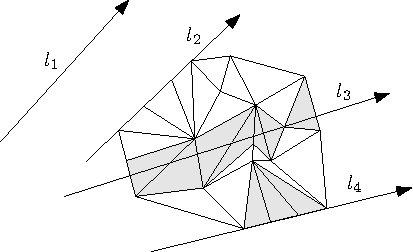
\includegraphics{Triangulation_2/walk} \end{center}
%\end{ccTexOnly} 
%
%
%\begin{ccHtmlOnly}
%<CENTER>
%<img border=0 src="./walk.gif" align=middle alt="The Infinite Vertex">
%</CENTER>
%\end{ccHtmlOnly} 
%
%\caption{The line face circulator.
%\label{Triangulation_ref_Fig_Line_face_circulator}}
%\end{figure}
%
%A line face circulator is invalidated if the face the circulator refers
%to is changed.
%
%

\ccHeading{Implementation}

Locate is implemented by a randomized walk from a vertex of the
face given as optional parameter (or from an arbitrary vertex of if no
optional parameter is given).

Insertion of a point is done by locating a face that contains the
point, and then splitting this face.  Apart from the location,
insertion takes a time $O(1)$.

Removal of a vertex is done by removing all adjacent triangles, and
re-triangulating the hole. Removal takes time $O(d^2)$ in the worst
case, if $d$ is the degree of the removed vertex, which is $O(1)$ for
a random vertex.

The face, edge, and vertex iterators on features are derived from
their counterparts visiting all (non-virtual and virtual) features
which are themselves derived from the corresponding iterators of the
triangulation data structure.



\ccSeeAlso
\ccc{Triangulation_2} \\
\ccc{Periodic_2TriangulationTraits_2} \\
\ccc{TriangulationDataStructure_2} \\
\ccc{TriangulationDataStructure_2::Face} \\
\ccc{TriangulationDataStructure_2::Vertex} \\
\ccc{CGAL::Triangulation_data_structure_2<Vb,Fb>} \\
\ccc{CGAL::Periodic_2_triangulation_face_base_2<Traits>}


%\ccExample

%The following code fragment creates a  triangulation of 2D points
%for the  usual Euclidean metric. The points are read from {\tt cin},
%inserted in the triangulation 
%and finally points on the convex hull are written to {\tt cout}. 
%\ccIncludeExampleCode{Triangulation_2/triangulation_prog1.cpp}


\end{ccRefClass}
\ccModifierCrossRefOn

% +------------------------------------------------------------------------+
%%RefPage: end of main body, begin of footer
% EOF
% +------------------------------------------------------------------------+

